%This work is licensed under the Creative Commons
%Attribution-ShareAlike 4.0 International License. To view a copy of
%this license, visit http://creativecommons.org/licenses/by-sa/4.0/ or
%send a letter to Creative Commons, PO Box 1866, Mountain View, CA
%94042, USA.

%This work is licensed under the Creative Commons
%Attribution-ShareAlike 4.0 International License. To view a copy of
%this license, visit http://creativecommons.org/licenses/by-sa/4.0/ or
%send a letter to Creative Commons, PO Box 1866, Mountain View, CA
%94042, USA.

%\documentclass[gray,handout, pdflatex, 11pt]{beamer}
%\documentclass[handout, pdflatex, 11pt]{beamer}

\documentclass[pdflatex, 11pt]{beamer}

\usepackage[utf8]{inputenc}
\usepackage[T1]{fontenc}
\usepackage{calligra}
\usepackage{lmodern}
%\usepackage[italian]{babel}
\usepackage{acronym}
\usepackage{graphicx}
\usepackage{multirow}
\usepackage{listings}
\usepackage{microtype}
\usepackage{acronym}
\usepackage{array}
\usepackage{pifont}
\usepackage{appendixnumberbeamer}
\usepackage{tikz}
\usetikzlibrary{shapes, chains, scopes, shadows, positioning, arrows,
  decorations.pathmorphing, calc, mindmap, petri}

\newcommand{\bigO}{\ensuremath{\mathcal{O}}}
\newcommand{\cmark}{\ding{52}}%{\ding{51}}
\newcommand{\xmark}{\ding{56}}%{\ding{55}}
\newcommand{\hmark}{\ding{42}}%{\ding{43}}
\newcommand{\ve}[1]{\ensuremath{\boldsymbol{#1}}}
\newcommand{\mE}{\ensuremath{\mathbb{E}}}
\newcommand{\mR}{\ensuremath{\mathbb{R}}}
\newcommand{\norm}[1]{\left\lVert#1\right\rVert_2}

\newcommand{\obsSet}{\ensuremath{O}}

\makeatletter
\newcommand{\pushright}[1]{\ifmeasuring@#1\else\omit\hfill$\displaystyle#1$\fi\ignorespaces}
\newcommand{\pushleft}[1]{\ifmeasuring@#1\else\omit$\displaystyle#1$\hfill\fi\ignorespaces}
\makeatother


\def\transW{8mm}
\def\transH{2mm}


\graphicspath{{img/}}

\definecolor{links}{HTML}{2A1B81}
\hypersetup{colorlinks,linkcolor=links,urlcolor=links}

\definecolor{links}{HTML}{2A1B81}
\hypersetup{colorlinks,linkcolor=,urlcolor=links}


\mode<presentation>{
  \usetheme{Martina}
  %-------------------------1
  %\usetheme{Boadilla}
  %\usecolortheme{beaver}
  %-------------------------1
  %-------------------------2
  %\usetheme{Goettingen}
  %\usecolortheme{sidebartab}
  %-------------------------2
  %\useoutertheme[right]{sidebar}
  %\usefonttheme{default}
  \setbeamercovered{transparent}
  %\setbeameroption{show notes on second screen=right}
  %\setbeamertemplate{navigation symbols}{}
  %\setbeamertemplate{footline}{}

  \bibliographystyle{abbrv}  
  %\renewcommand\bibfont{\scriptsize}
  \setbeamertemplate{bibliography item}{\textbullet}
  \setbeamertemplate{itemize item}{\cmark}
  % \setbeamertemplate{itemize subitem}{-}
  \setbeamertemplate{enumerate items}[default]
  \setbeamertemplate{sections/subsections in toc}[square]
}

% \usebackgroundtemplate
% {
%   \begin{tikzpicture}
%     \node[opacity=0.1] {
\includegraphics[]{img/logoUnifi.png}};
% %    \node[opacity=0.04] {
\includegraphics[scale=1]{img/logoUnifi.eps}};
%   \end{tikzpicture}
% }


\begin{document}

\title[]{\textbf{Fuzzy logic course}\\ \tiny{(Beatrice Lazzerini, Uni. Pisa)}\\
  \tiny{Atin\c{c} Ylmaz,
    Se\c{c}kin Aria, \"{U}mit Kocabi\c{c}ak,}\small{\textbf{Risk analysis of lung
    cancer and effects of stress 
    level on cancer risk through neuro-fuzzy model},}\\
  \tiny{Computer methods and programs in biomedicine 137 (2016) 35-46}}
\date[17 May 2017]{17 May 2017}
%\subtitle{Master degree thesis}
\institute[Uni. Firenze]{
  
\includegraphics[width=5cm]{img/logoUnifiName.eps}
}

\author[Martina Stefano]{
  \begin{center}
    \begin{tabular}{lr}
      Stefano \textsc{Martina}\\
      \href{mailto:stefano.martina@unifi.it}{stefano.martina@unifi.it}\\
    \end{tabular}
  \end{center}
}

% \titlegraphic{
%   \vspace{-0.5cm}
%   \tiny
%   \href{http://creativecommons.org/licenses/by-sa/4.0/}{
\includegraphics[width=1cm]{img/logoCC.png}}
%   This work is licensed under a
%   \href{http://creativecommons.org/licenses/by-sa/4.0/}{Creative
%     Commons Attribution-ShareAlike 4.0 International License}.
% }

\newacro{ANFIS}{Adaptive neuro-fuzzy inference system}

\begin{frame}[plain]
  \titlepage
\end{frame}

\begin{frame}{Fuzzy logic in medicine}
  \begin{itemize}
  \item \alert{insufficient} information\pause
  \item provided information is \alert{subjective}\pause
  \item unclear \alert{border} between healthy and pathological\pause
  \item \alert{errors} and misconducts on diagnostic tests\pause
  \item \alert{faked} symptoms\pause
  \item \alert{limited} experiments (1536 subjects in this)
  \end{itemize}
\end{frame}

\begin{frame}{\acf{ANFIS}}
  Unifies decision ability and verbal expression of fuzzy logic with
  learning ability and adaptivity of neural networks.
  \begin{center}
    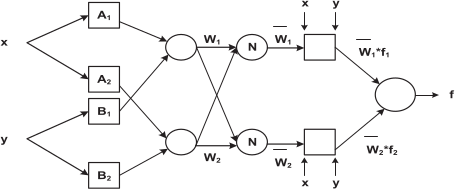
\includegraphics[width=0.6\textwidth]{img/anfis.png}
  \end{center}
  \pause
  \begin{itemize}
  \item Layer 1 is \alert{input}\pause
  \item Layer 2 \alert{cluster membership} degree (least squares)\pause
  \item Layer 3 are the \alert{rules} (different t-norms)\pause
  \item Layer 4 is \alert{normalization}\pause
  \item Layer 5 is \alert{defuzzification} (backpropagation)\pause
  \item Layer 6 is \alert{output}
  \end{itemize}
\end{frame}

\begin{frame}{Intersection operators}
  \begin{center}
    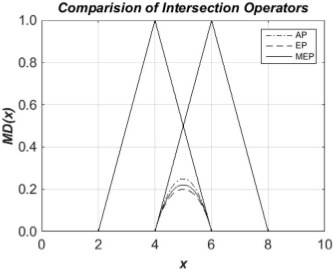
\includegraphics[width=0.4\textwidth]{img/operators.png}
  \end{center}
  \begin{itemize}
  \item \alert{Algebraic product} $\mu_{A_i}(x)\mu_{B_i}(y)\dots \mu_{T_i}(t)$\pause
  \item \alert{Einstein product} $\frac{\mu_{A_i}(x)\mu_{B_i}(y)}{1+(1-\mu_{A_i}(x))((1-\mu_{B_i}(y)))}$\pause
  \item \alert{Modified Einstein product}
    $\frac{K\mu_{A_i}(x)\mu_{B_i}(y)\dots\mu_{K_i}(k)}{K+(1-\mu_{A_i}(x))((1-\mu_{B_i}(y))\dots
      ((1-\mu_{K_i}(k)))}$\pause
    \begin{itemize}
    \item converges to algebraic product
    \end{itemize}
  \end{itemize}
\end{frame}

\begin{frame}{Cancer model}
  \begin{center}
    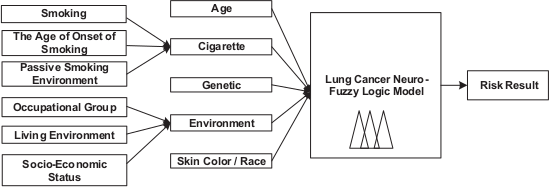
\includegraphics[width=0.5\textwidth]{img/cancerModel.png}\hspace{0.5cm}
    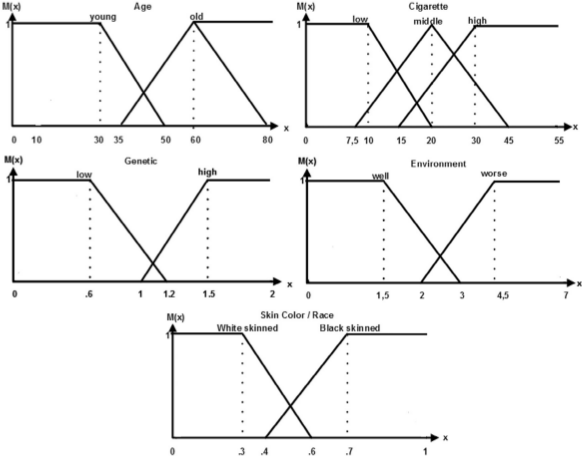
\includegraphics[width=0.4\textwidth]{img/cancerMember.png}\\[0.5cm]
    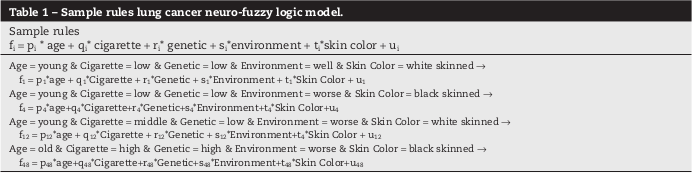
\includegraphics[width=0.8\textwidth]{img/cancerRules.png}
  \end{center}
\end{frame}

\begin{frame}{Stress model}
  \begin{center}
    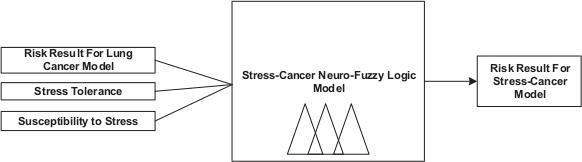
\includegraphics[width=0.5\textwidth]{img/stressModel.png}\hspace{0.5cm}
    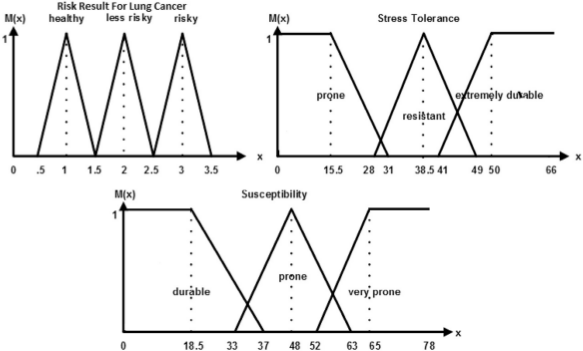
\includegraphics[width=0.4\textwidth]{img/stressMember.png}\\[0.5cm]
    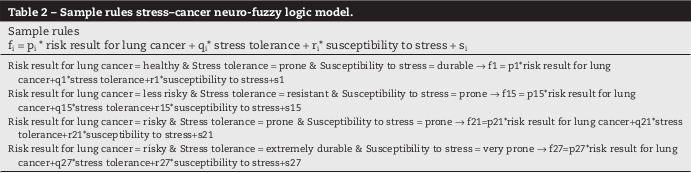
\includegraphics[width=0.8\textwidth]{img/stressRules.png}
  \end{center}
\end{frame}

\begin{frame}{Results}
  \begin{center}
    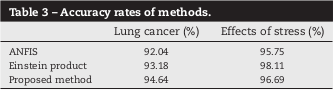
\includegraphics[width=0.4\textwidth]{img/accuracy.png}\\[0.5cm]
    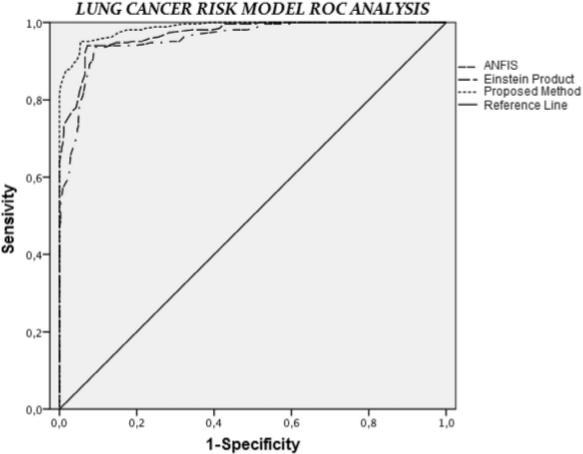
\includegraphics[width=0.6\textwidth]{img/roc.png}
  \end{center}
\end{frame}


\end{document}

%%% Local Variables:
%%% mode: latex
%%% TeX-master: t
%%% End:
